\documentclass[xcolor=table]{beamer}
\usepackage{graphicx}
\usepackage[spanish]{babel} % para escribir en espanol
\usepackage[utf8]{inputenc}
\usepackage{wrapfig}

\graphicspath{ {imagenes/} }

\usetheme{Madrid}

\title{Aplicaciones del análisis multivariante con R}
\subtitle{Estadística Multivariante - Universidad de Granada}

\author{Laura Gómez Garrido\\ Miguel Lentisco Ballesteros \\ Antonio Martín Ruiz \\ Daniel Pozo Escalona \\Francisco Javier Sáez Maldonado}

\AtBeginSection[]
{
  \begin{frame}<beamer>{}
    \tableofcontents[currentsection,currentsubsection]
  \end{frame}
}

\begin{document}
\begin{frame}
\titlepage
\end{frame}
\begin{frame}{Contenido}
  \tableofcontents
  % You might wish to add the option [pausesections]
\end{frame}
\section{Introducción: R}

\begin{frame}{¿Qué es R?}

R es un entorno y lenguaje de programación enfocados a la computación estadística y de gráficos. Surge como una reimplementación libre del lenguaje y entorno S. Proporciona una amplia variedad de funcionalidades estadísticas y gráficas y es altamente extensible.
\newline
\newline
R está disponible como software libre bajo los términos de la GNU General Public License de la Free Software Foundation en forma de código fuente. Puede ser compilado y ejecutado en una gran cantidad de plataformas UNIX, Windows y MacOs.

\end{frame}

\begin{frame}{Entornos de desarrollo para R}
\end{frame}

\begin{frame}{Principales librerías}

\end{frame}

\begin{frame}{Algunas aplicaciones de R}
\end{frame}

\section{R en el análisis multivariante}
\begin{frame}{Nuestro dataset}

\begin{table}[]
\resizebox{10cm}{!}{
\begin{tabular}{|
>{\columncolor[HTML]{979CD8}}l |l|
>{\columncolor[HTML]{979CD8}}l |l|}
\hline
\textbf{Característica del data set}      & Multivariante   & \textbf{Nº de Instancias} & 178        \\ \hline
\textbf{Características de los atributos} & Enteros, Reales & \textbf{Nº de Atributos}  & 13         \\ \hline
\textbf{Área}                             & Física          & \textbf{Donado}           & 01/07/1991 \\ \hline
\end{tabular}
}
\end{table}
\begin{wrapfigure}{r}{0.25\textwidth}
\centering
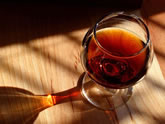
\includegraphics[width=0.25\textwidth]{vino.jpg}
\end{wrapfigure}
{Fuente: Machine Learning Repository\\
Propietarios Originales: }\begin{quote}\scriptsize Forina, M. et al, PARVUS -\\
An Extendible Package for Data Exploration, Classification \\and Correlation.\\
Institute of Pharmaceutical and Food Analysis and Technologies, \\Via Brigata Salerno,
16147 Genoa, Italy.\end{quote}
\end{frame}


\subsection{Distribución Normal Multivariante. Ejemplos}

\begin{frame}{Lectura y media}
\begin{lstlisting}
wine <- read.table("http://archive.ics.uci.edu/ml/machine-learning-databases/wine/wine.data",sep=","); wine
\end{lstlisting}
\begin{wrapfigure}{r}{0.25\textwidth}
\centering
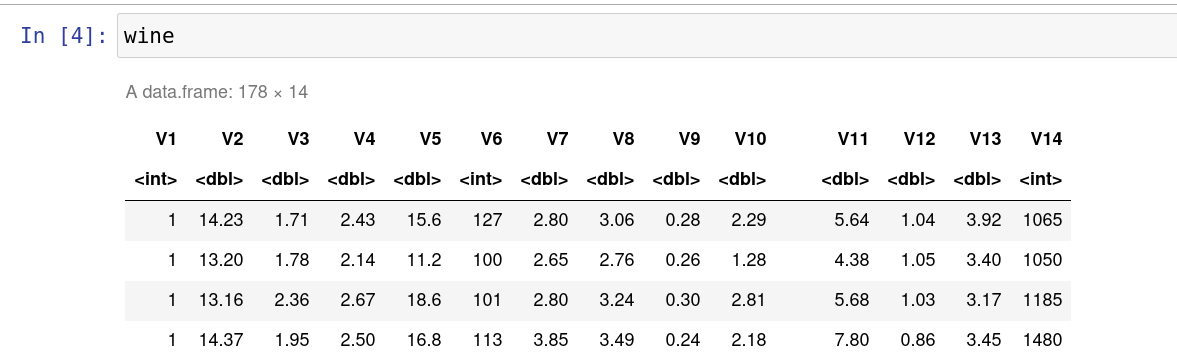
\includegraphics[width=0.25\textwidth]{dataframe_wine.png}
\end{wrapfigure}
\begin{lstlisting}
sapply(wine[2:14],mean)
"Media muestral del conjunto completo"

V2
    13.0006179775281
V3
    2.33634831460674
V4
    2.36651685393258
V5
    19.4949438202247
V6
    99.7415730337079
V7
    2.29511235955056
V8
    2.02926966292135
V9
    0.36185393258427
V10
    1.59089887640449
V11
    5.05808988202247
V12
    0.957449438202247
V13
    2.61168539325843
V14
    746.893258426966
    
\end{lstlisting}

\end{frame}
\begin{frame}{Dibujado de datos seleccionados. Scatterplots}
\begin{lstlisting}
selection1 <- wine[wine$V1 == "1",]
selection3 <- wine[wine$V1 == "3",]
mean1 <- sapply(selection1[2:14],mean)
mean2 <- sapply(selection3[2:14],mean)
chemical <- c(2,3,4,5,6,7,8,9,10,11,12,13,14)
plot(chemical,mean1,col = "red")
points(chemical, mean2, col="blue", pch="*")
legend(2,1000,legend=c("Medias en Fabrica 1","Medias en Fabrica 2"), col=c("red","blue"),
                                   pch=c("o","*"))
\end{lstlisting}
\begin{wrapfigure}{r}{0.25\textwidth}
\centering
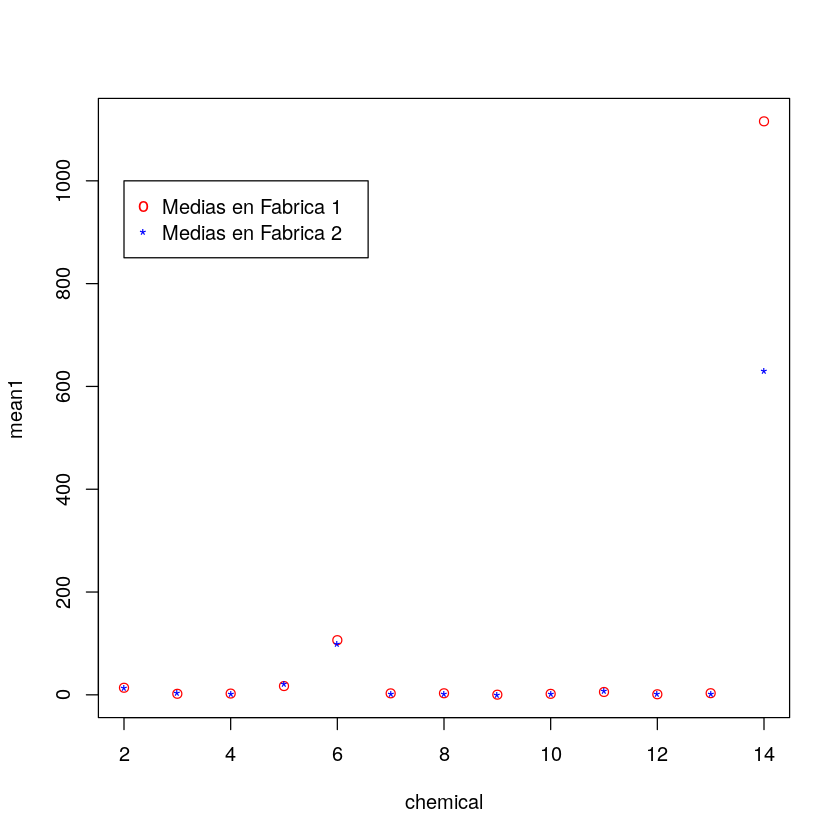
\includegraphics[width=0.25\textwidth]{means.png}
\end{wrapfigure}
Podemos realizar scatterplots de la siguiente manera
\begin{lstlisting}
plot(popul ~ manu, data = USairpollution)
\end{lstlisting}
\begin{wrapfigure}{r}{0.25\textwidth}
\centering
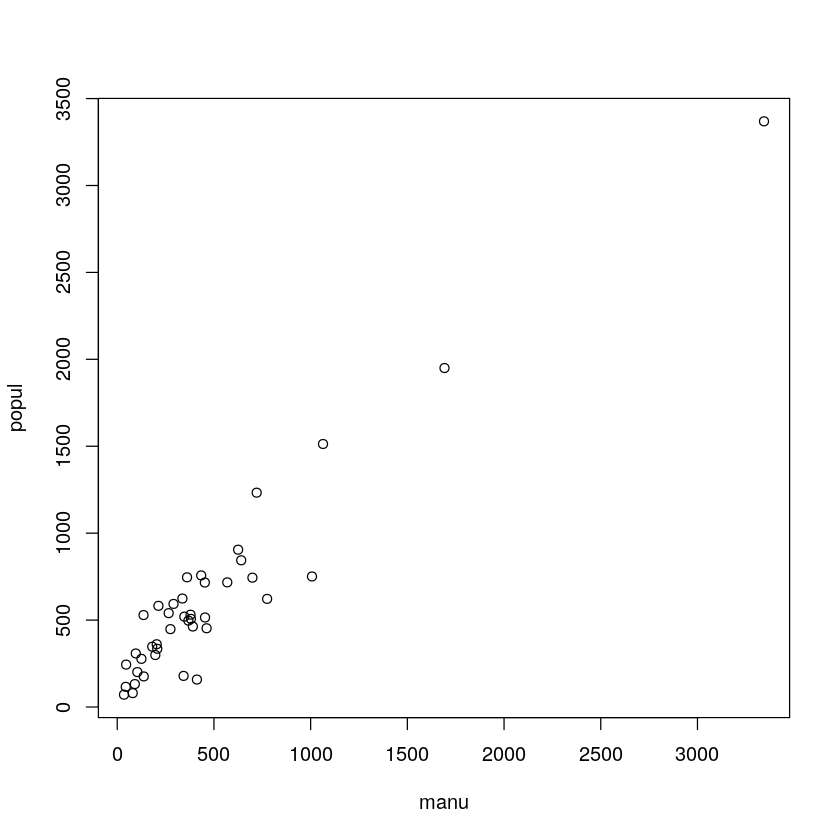
\includegraphics[width=0.25\textwidth]{scatter.png}
\end{wrapfigure}
O, dibujar todas las parejas posibles a la vez, y añadir las rectas de regresión
\begin{lstlisting}
pairs(USairpollution,
     panel = function(x, y, ...) {
         points(x, y, ...)
         abline(lm(y ~ x), col = "grey")
     }, pch = ".", cex = 1.5)
\end{lstlisting}
\begin{wrapfigure}{r}{0.25\textwidth}
\centering
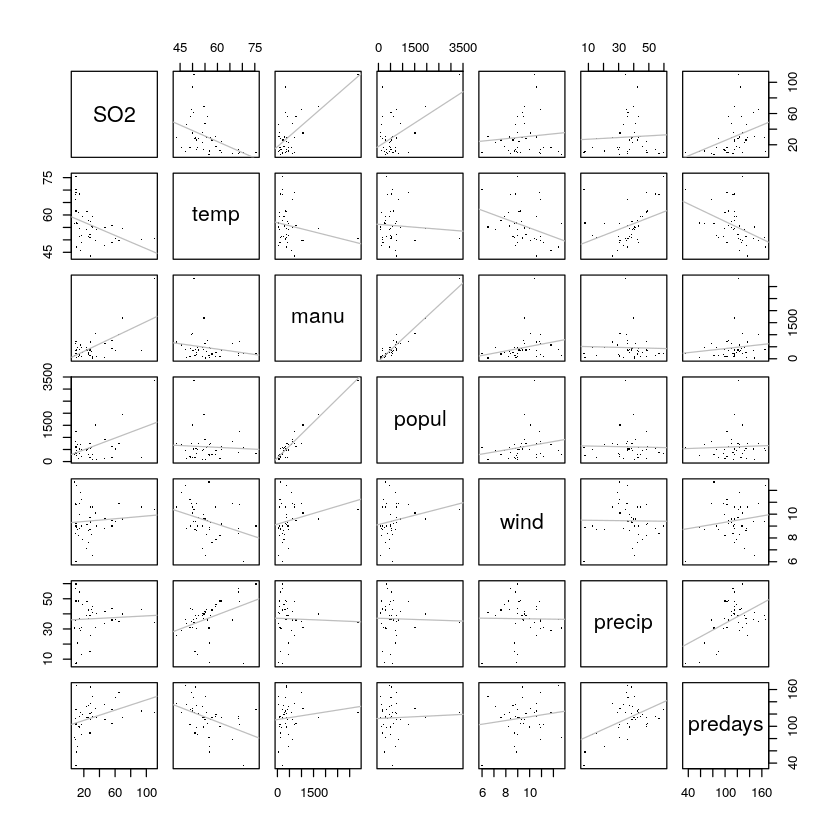
\includegraphics[width=0.25\textwidth]{reg.png}
\end{wrapfigure}
\end{frame}

\begin{frame}{Implementación Teórica de una DNM}

\begin{listings}
DNM <- setRefClass("DNM", 
                   fields = list(p = "numeric", 
                                 media = "matrix", 
                                 cov = "matrix"))
\end{listings}
\end{frame}

\section{Para ampliar}
\begin{frame}{Para ampliar}
\textit{Computing Machinery and Intelligence} Alan Turing (1950)
\newline
\newline
\textit{Artifficial Intelligence: A Modern Aproach} Stuart J. Russell y Peter Norvig
\newline
\newline
\textit{Concrete Problems in AI Safety} Dario Amodei, Crhis Olah, Jacob Steinahrdt, Paul Christiano, John Schulman, Dan Mané
\newline
\newline
\textit{The Malicious Use of Artificial Intelligence: Forecasting, Prevention, and Mitigation} Miles Brundage, Shahar Avin et al.
\end{frame}
\end{document}
